% https://tex.stackexchange.com/a/369484/173708
\documentclass[margin=10pt]{standalone}
\usepackage{tikz}

\usetikzlibrary{
    shapes.geometric
    ,positioning
}
\tikzset{
    zeitmarkernode/.style={
        isosceles triangle
        ,minimum height=2.5mm
        ,inner sep=0pt
        ,anchor=apex
    },
    zeitmarker/.pic={%
        \node[zeitmarkernode,pic actions,rotate=-90](-o){};
        \node[zeitmarkernode,pic actions,rotate=90](-u){};
    }
}
\begin{document}
    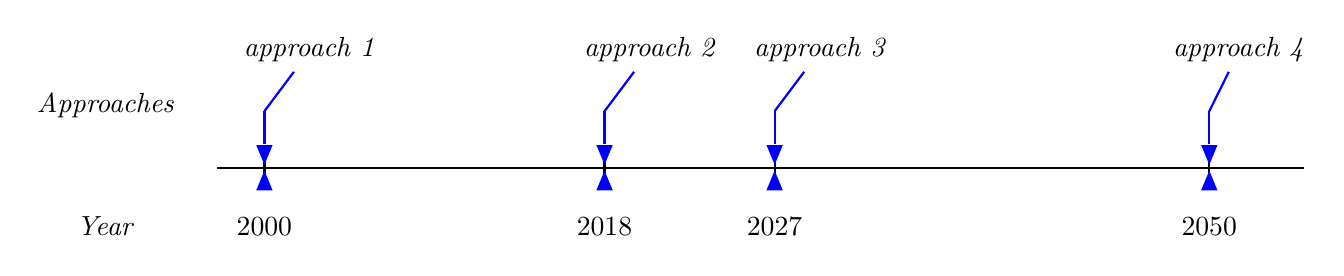
\begin{tikzpicture}[x=6cm,thick]
    % Achse und Beschriftung unterhalb
    \draw (11.9,0) -- (12,0) coordinate (s) -- (12+18/25,0) coordinate (a) 
        -- (12+27/25,0) coordinate (b) -- (14,0) coordinate (e) -- (14.2,0);
    \foreach \c/\zeit in {s/2000,a/2018,b/2027,e/2050}
        \draw (\c) node[below=.5cm of \c] {\zeit} -- +(0,.1) -- +(0,-.1);

    % Markierungen, Beschriftungen oberhalb und Verbindungen
    \foreach[count=\i] \descr/\c/\hshift in {%
        approach 1/s/5mm,%
        approach 2/a/5mm,%
        approach 3/b/5mm,%
        approach 4/e/3mm%
    }{
        \pic[fill=blue] (zm\i) at (\c) {zeitmarker};
        \node[above=1cm of zm\i-o,xshift=\hshift] (zm\i) {\emph{\descr}};
        \coordinate(h) at ([yshift=5mm]zm\i-o);
        \draw[blue](h) edge (zm\i) edge (zm\i-o);
    }
    \node[below left =.5cm and 1cm of s, text width=5em, align=center, text height=1.5ex,text depth=.25ex] {\emph{Year}};
    \node[above left =.5cm and 1cm of s, text width=5em, align=center] {\emph{Approaches}};
    \end{tikzpicture}
\end{document}